\section{ARP}

\begin{center}
    \begin{tikzpicture}[
            node distance = 1mm and 0mm,
            start chain = going below,
            desc/.style args = {#1/#2}{
                    rectangle, rounded corners, draw, very thick,
                    text width=8cm, align=center,
                    fill=theme-2!#1,
                    minimum height=12mm,
                    label=left:Layer #2,
                    on chain
                },
            level/.style = {
                    rectangle, rounded corners, draw, very thick,
                    fill=theme-1!#1
                    text width=3cm, align=center,
                    minimum height=12mm
                },
        ]
        \node   [desc=0/7]     {Applications layer};
        \node   [desc=0/6]     {Presentation layer};
        \node   [desc=0/5]     {Session layer};
        \node   [desc=0/4]     {Transport layer};
        \node   [desc=0/3]     {Network layer};
        \node   [desc=30/2]    {Data link layer};
        \node   [desc=0/1]     {Physical layer};
    \end{tikzpicture}
\end{center}


How does a host find out the MAC address of another host on the same
network?  The answer is the Address Resolution Protocol (ARP).  ARP is
a protocol that allows a host to find out the MAC address of another
host on the same network.

\subsection{Topology}

The topology for this section is shown in Figure~\ref{fig:arp-topology}.

\begin{figure}
    \centering
    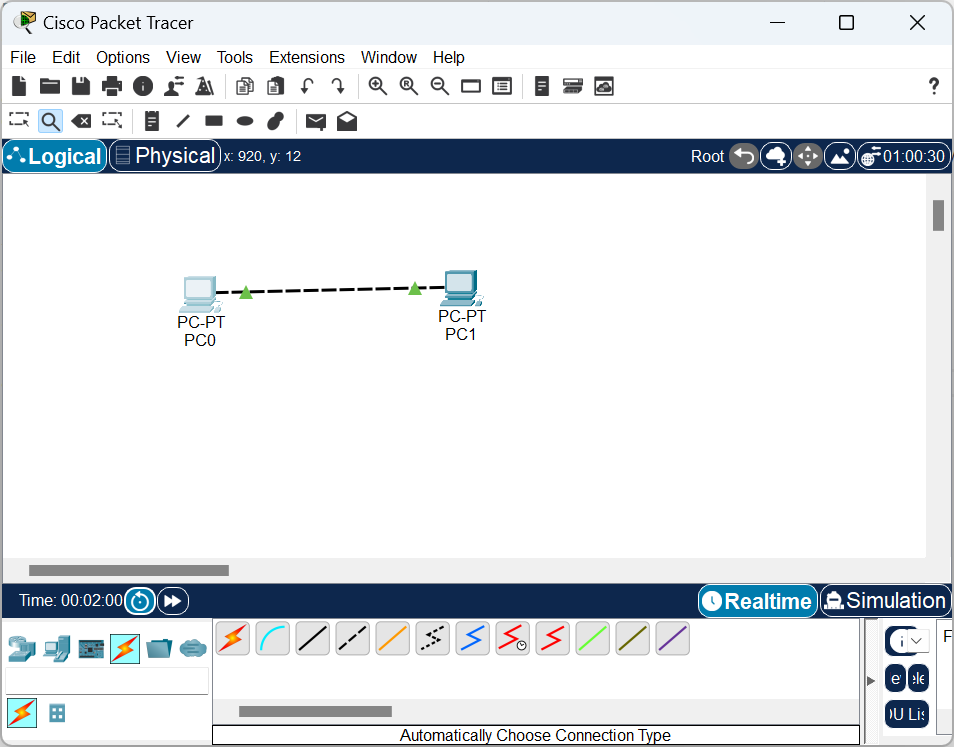
\includegraphics[width=0.5\textwidth]{images/arp-topology.png}
    \caption{ARP Topology}\label{fig:arp-topology}
\end{figure}

It consists of 2 computers with IP address \mono!192.168.0.1! and
\mono!192.168.0.2! respecitvely. Two computers are connected with
copper cross over cable directly.

Use \menu{inspect} \icon{inspect} tool to inspect the ARP table, and we would
see that there is clearly nothing, as shown at \autoref{fig:arp-inspect}.

\begin{figure}[!htbp]
    \centering
    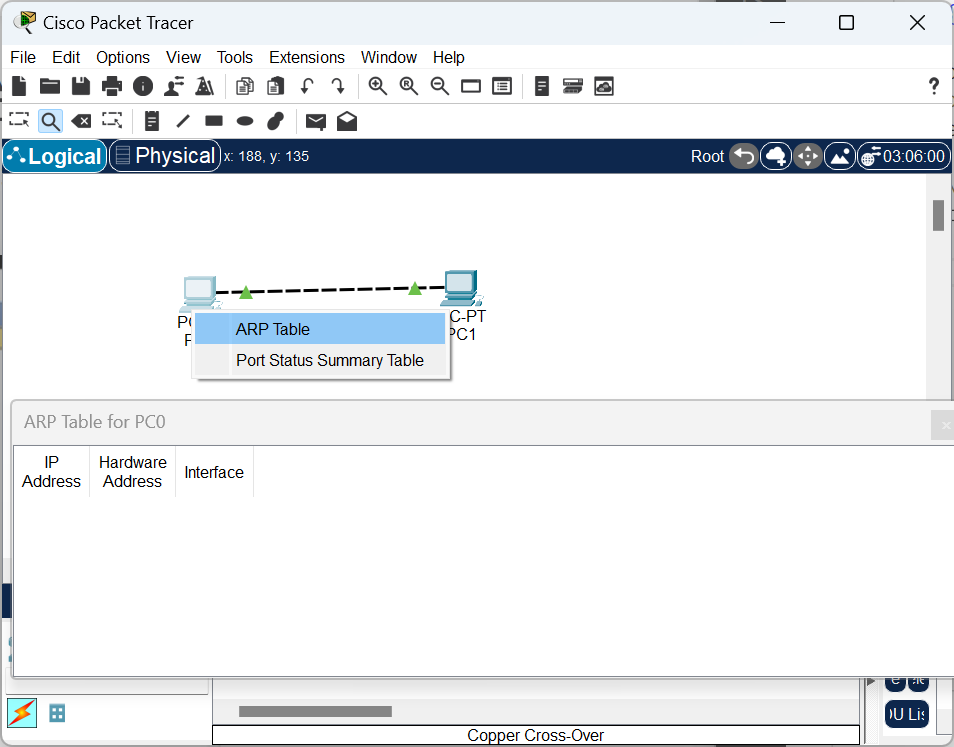
\includegraphics[width=0.5\textwidth]{images/arp-inspect.png}
    \caption{ARP Inspect}\label{fig:arp-inspect}
\end{figure}

While we are setting the IP address, open the simulation mode. After the IP
address has been set, we would see the ARP table is filled with the MAC address
of the other host.

\begin{figure}[!htbp]
    \centering
    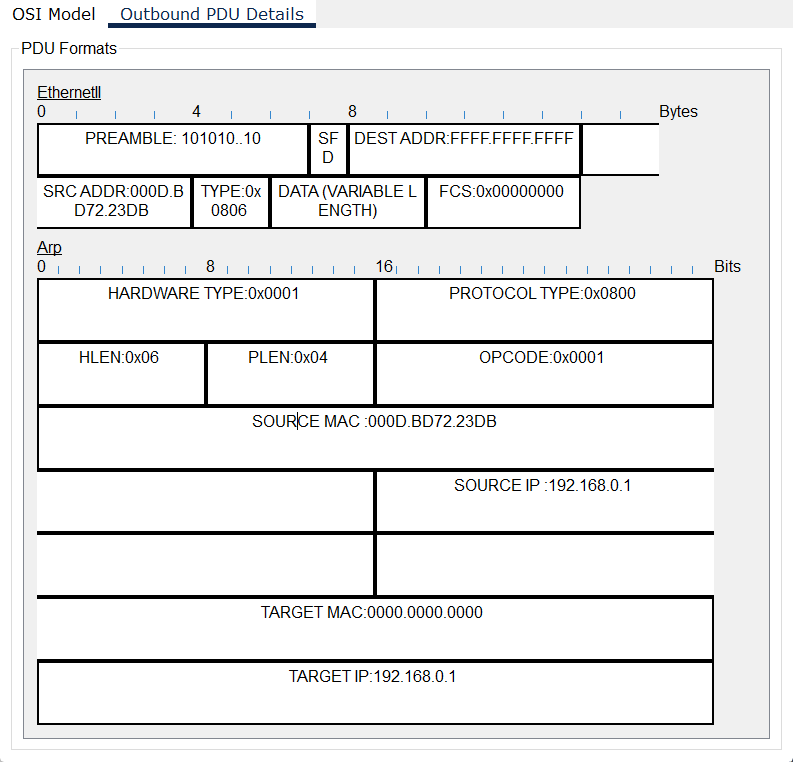
\includegraphics[width=0.5\textwidth]{images/arp-req.png}
    \caption{ARP Packet Structure}\label{fig:arp-req}
\end{figure}

Computer resolves the MAC address of the other host by sending an ARP request
packet to the broadcast address with structure shwon at \autoref{fig:arp-req}.

\begin{description}
    \item[Hardware Type] \mono!1! indicates Ethernet.
    \item[Protocol Type] \mono!0x0800! indicates IPv4.
    \item[Hlen] \mono!6! indicates the length of the hardware address (octets).
    \item[Plen] \mono!4! indicates the length of the protocol address (octets).
    \item[Operation] \mono!1! indicates ARP request.
    \item[Source MAC] is the MAC address of the sender.
    \item[Source IP] is the IP address of the sender.
    \item[Targer MAC] is the MAC address of the target. Notice because the
        computer \emph{does not know} the MAC address of the target, it is set to
        \mono!0000:0000:0000!, representing the \emph{boardcast address} or
        \emph{multi-cast address}.
    \item[Target IP] is the IP address of the target.
\end{description}

When the target receives the ARP request, it will send an ARP reply packet to
the sender. Further, it will also update its ARP table with the sender's MAC
address, with structure shown at \autoref{fig:arp-reply}.

\begin{figure}[!htbp]
    \centering
    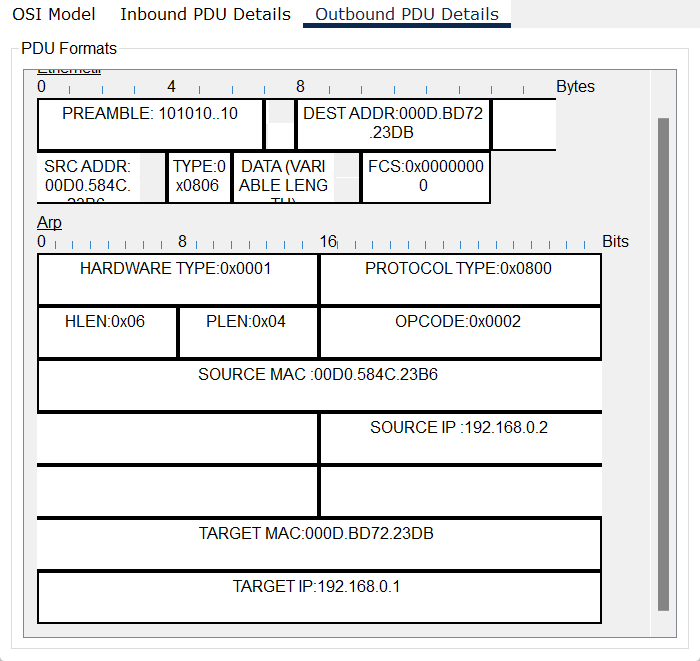
\includegraphics[width=0.5\textwidth]{images/arp-reply.png}
    \caption{ARP Packet Structure}\label{fig:arp-reply}
\end{figure}

After the ARP cache table has been updated, the sender can send data packets to
the target. ARP table is regularly updated by sending ARP request packets in a
specific interval, called \emph{ARP timeout}. In Cisco Packet Tracer, the
default ARP timeout is 14400 seconds.

In order to clear, or display ARP information using commandline, click on any
PC and open \menu{Desktop > Command Prompt}. Type \mono!arp -a! to display
the ARP table, and type \mono!arp -d! to clear the ARP table, as shown at \autoref{fig:arp-cmd}.

\begin{figure}
    \centering
    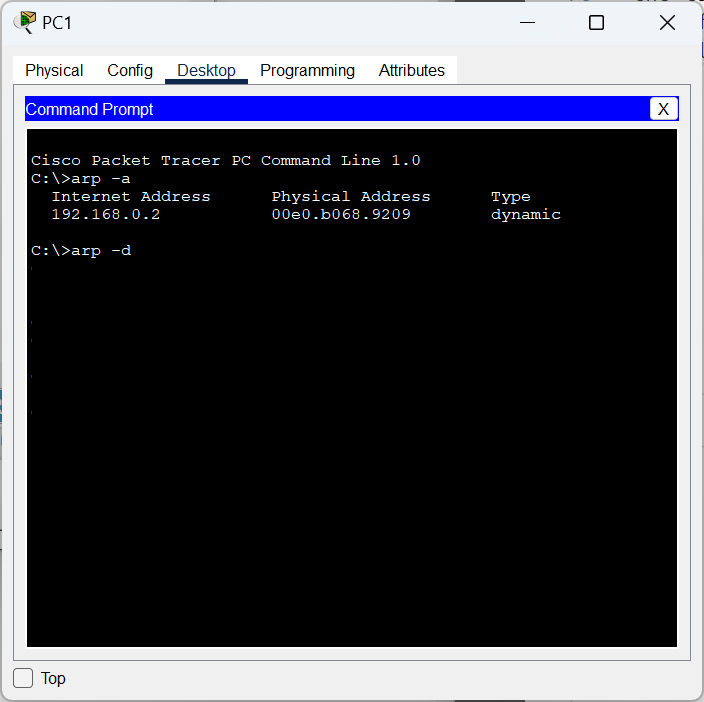
\includegraphics[width=0.5\textwidth]{images/arp-cmd.png}
    \caption{ARP Command}\label{fig:arp-cmd}
\end{figure}

